\section{问题二的建模与求解}
\label{sec:problem2}
\subsection{模型建立}
在问题一得到的可行非支配方案中，以碳排放、成本和强度为评价指标。
根据实际决策需求确定归一化方式、权重或优先级，建立折中方案选择模型。

\subsection{求解与结果分析}
表~\ref{tab:results}展示结果表格式，“待填”应替换为实际计算值。
结合式~\eqref{eq:objectives}解释目标取舍、方案选择依据与约束满足情况。
\begin{table}[!htb]
  \centering
  \caption{方案比较（结果待填写）}
  \label{tab:results}
  \begin{tabular}{@{}lccc@{}}
    \toprule
    方案 & 碳排/(kg CO$_2$e/m$^3$) & 成本/(元/m$^3$) & 强度/MPa\\
    \midrule
    基准方案 & 待填 & 待填 & 待填\\
    折中方案 & 待填 & 待填 & 待填\\
    \bottomrule
  \end{tabular}
\end{table}

图~\ref{fig:example}是一幅使用合成数据制作的静态示例图，仅用于展示插图格式。
使用时替换图片文件、图题及相应说明。
\begin{figure}[H]
  \centering
  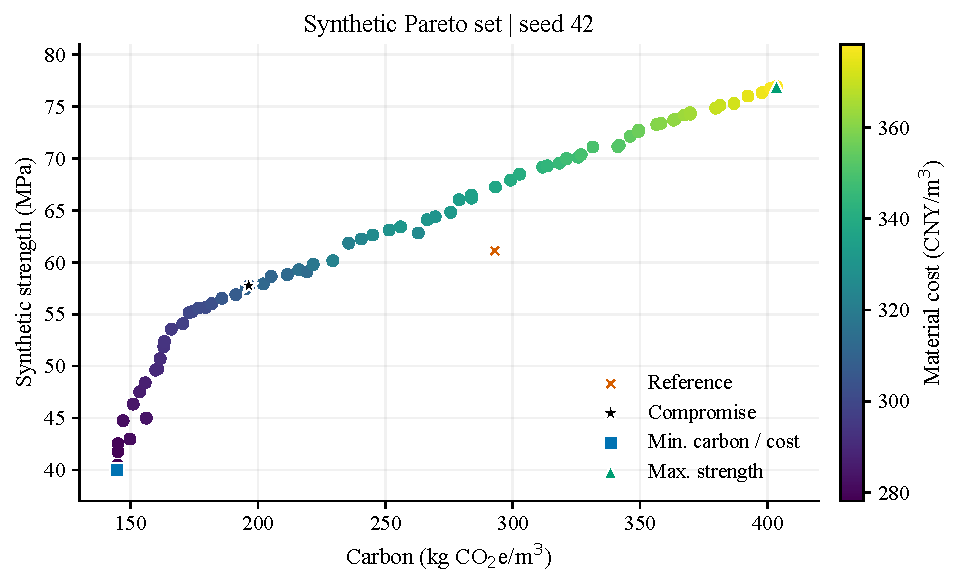
\includegraphics[width=0.72\linewidth]{figures/example-plot.pdf}
  \caption{静态插图示例（合成数据）}
  \label{fig:example}
\end{figure}
